\documentclass[12pt, letterpaper]{article}

% ── Packages ──────────────────────────────────────────────────────────────────
\usepackage[T1]{fontenc}
\usepackage[utf8]{inputenc}
\usepackage[margin=1.25in]{geometry}
\usepackage{booktabs}
\usepackage{array}
\usepackage{tabularx}
\usepackage{longtable}
\usepackage{enumitem}
\usepackage{hyperref}
\usepackage{xcolor}
\usepackage{titlesec}
\usepackage{parskip}
\usepackage{setspace}
\usepackage{graphicx}
\usepackage{float}
\usepackage{caption}
\usepackage{mdframed}
\usepackage{tcolorbox}
\usepackage{fancyhdr}
\usepackage{needspace}
\usepackage{amsmath}
\usepackage{amssymb}
\usepackage{multicol}   % two-column TOC
\usepackage{tikz}       % for system architecture diagram
\usetikzlibrary{shapes, arrows, positioning, shadows}
\setlength{\headheight}{25pt}
\addtolength{\topmargin}{-10pt}

% ── Colours ───────────────────────────────────────────────────────────────────
\definecolor{primary}{HTML}{1F4E79}
\definecolor{accent}{HTML}{2E75B6}
\definecolor{lightblue}{HTML}{D5E8F0}
\definecolor{codebg}{HTML}{F5F5F5}
\definecolor{muted}{HTML}{555555}

% ── Hyperref setup ────────────────────────────────────────────────────────────
\hypersetup{
  colorlinks  = true,
  linkcolor   = accent,
  urlcolor    = accent,
  citecolor   = accent,
  pdftitle    = {SearchVision White Paper},
  pdfauthor   = {Brandon Shen},
  pdfsubject  = {Human-in-the-Loop Object Detection Dataset Generation from Web Images},
  pdfkeywords = {object detection, YOLOv8, computer vision, machine learning, web scraping},
}

% ── Section heading styles ────────────────────────────────────────────────────
\titleformat{\section}
  {\Large\bfseries\color{primary}}
  {\thesection.}{0.6em}{}
  [\vspace{-0.3em}\textcolor{accent}{\rule{\linewidth}{1.5pt}}\vspace{0.3em}]

\titleformat{\subsection}
  {\large\bfseries\color{accent}}
  {\thesubsection}{0.6em}{}

\titleformat{\subsubsection}
  {\normalsize\bfseries\color{muted}}
  {\thesubsubsection}{0.5em}{}

\titlespacing*{\section}{0pt}{1.5em}{0.8em}
\titlespacing*{\subsection}{0pt}{1.2em}{0.5em}
\titlespacing*{\subsubsection}{0pt}{1em}{0.3em}

% ── Page style ────────────────────────────────────────────────────────────────
\pagestyle{fancy}
\fancyhf{}
\fancyhead[L]{\small\textcolor{muted}{SearchVision \textemdash\ White Paper}}
\fancyhead[R]{\small\textcolor{muted}{v1.1}}
\fancyfoot[C]{\small\textcolor{muted}{\thepage}}
\renewcommand{\headrulewidth}{0.4pt}
\renewcommand{\headrule}{\hbox to\headwidth{%
  \color{accent}\leaders\hrule height \headrulewidth\hfill}}
\renewcommand{\footrulewidth}{0pt}

% ── Table / caption style ─────────────────────────────────────────────────────
\captionsetup{font=small, labelfont={bf,color=primary}, skip=6pt}
\setlength{\extrarowheight}{3pt}

% ── List style ────────────────────────────────────────────────────────────────
\setlist[itemize]{itemsep=2pt, topsep=4pt, leftmargin=1.5em}
\setlist[enumerate]{itemsep=2pt, topsep=4pt, leftmargin=1.5em}

% ── Inline code ───────────────────────────────────────────────────────────────
\newcommand{\code}[1]{\texttt{\small\colorbox{codebg}{#1}}}

% ── Info box ──────────────────────────────────────────────────────────────────
\tcbuselibrary{skins}
\newtcolorbox{infobox}[1][]{
  colback  = lightblue!40,
  colframe = accent,
  fonttitle= \bfseries\color{primary},
  boxrule  = 0.8pt,
  arc      = 3pt,
  left=8pt, right=8pt, top=6pt, bottom=6pt,
  #1
}

% ── Two-column TOC ───────────────────────────────────────────────────────────
% Redefine \tableofcontents to use two columns
\let\origtableofcontents\tableofcontents
\renewcommand{\tableofcontents}{%
  \begin{multicols}{2}[\origtableofcontents]
  \end{multicols}%
}

% ══════════════════════════════════════════════════════════════════════════════
\begin{document}
% ══════════════════════════════════════════════════════════════════════════════

% ── Cover page ────────────────────────────────────────────────────────────────
\pagenumbering{roman}
\begin{titlepage}
  \centering
  \vspace*{3cm}
  {\fontsize{48}{56}\selectfont\bfseries\color{primary} SearchVision}\\[0.8em]
  \textcolor{accent}{\rule{0.6\linewidth}{2pt}}\\[1em]
  {\Large\color{muted} Human-in-the-Loop Object Detection Dataset Generation}\\[0.3em]
  {\Large\color{muted} from Web Images}\\[2em]
  {\large\itshape White Paper \textemdash\ v1.1}\\[0.5em]
  {\normalsize\color{muted} Brandon Shen}\\[0.3em]
  {\normalsize\color{muted} July 2026}\\[3em]
  \textcolor{accent}{\rule{0.3\linewidth}{0.8pt}}\\[1.5em]
  {\small\color{muted}
    Licensed under AGPL-3.0 \quad\textbullet\quad
    Open-Source \quad\textbullet\quad
    \url{https://github.com/Brandon-Shen/SearchVision}
  }
  \vfill
\end{titlepage}

% ── Abstract ──────────────────────────────────────────────────────────────────
\begin{abstract}
SearchVision is a web-based platform that enables users to create custom object detection
models without writing code. By integrating web search (with intelligent fallback strategies),
automated web scraping, intelligent annotation workflows, and YOLOv8 model training into a 
unified workflow, SearchVision automates the traditionally labor-intensive process of dataset 
collection, annotation, and model training. Unlike existing solutions that focus on individual 
pipeline stages, SearchVision integrates all five stages---search, selection, annotation, 
scraping, and training---into a single interface. The system features a hybrid image selection 
algorithm combining search rank, caption relevance, and visual diversity; validated image downloads;
a held-out validation split; and conservative dataset augmentation using a pre-trained YOLOv8 model.
Google Custom Search is optional because an original-resolution Bing Images fallback is provided.
This whitepaper presents the system's architecture, feature set, technology stack, and practical 
use cases, while also acknowledging current limitations.
\end{abstract}

% ── Table of Contents (two-column, roman numerals) ────────────────────────────
\tableofcontents
\clearpage

% ── Switch to arabic numbering from here ─────────────────────────────────────
\pagenumbering{arabic}

% ══════════════════════════════════════════════════════════════════════════════
\section{Introduction}
% ══════════════════════════════════════════════════════════════════════════════

The proliferation of deep learning-based computer vision has enabled remarkable advances
in object detection, with applications spanning autonomous vehicles, medical imaging,
retail analytics, and industrial quality control. State-of-the-art models such as YOLO
\cite{redmon2018yolov3}, Faster R-CNN \cite{ren2015faster}, and their successors achieve
strong performance on standard benchmarks. However, the deployment of these models to
real-world problems remains challenging, particularly for practitioners outside of
well-resourced research laboratories.

The primary bottleneck is not the model architecture itself, but rather the dataset required
for training. Creating a custom object detection dataset involves four distinct challenges:
(1)~collecting relevant images, (2)~annotating those images with bounding boxes,
(3)~ensuring dataset diversity and quality, and (4)~configuring and executing the training
pipeline. Each step traditionally requires specialized tools, domain expertise, and
significant manual effort.

Several commercial and open-source solutions have emerged to address individual components
of this workflow. Annotation platforms such as CVAT \cite{cvat}, Label Studio
\cite{labelstudio}, and Roboflow \cite{roboflow} provide sophisticated interfaces for
bounding box creation. AutoML services from major cloud providers automate model training
but at substantial cost. SearchVision contributes a compact, open-source integration of
these stages rather than claiming that comparable integrated platforms do not exist.

This whitepaper presents SearchVision, a system that automates the complete object detection
dataset creation and model training workflow. The system accepts a text query from the user,
retrieves relevant images via web search, applies diversity-aware selection algorithms to
ensure dataset variety, expands the dataset through automated web scraping, supports both
manual and auto-annotation workflows, and trains a custom YOLOv8 model \cite{yolov8} with a
single click. By abstracting implementation details, SearchVision enables practitioners to
focus on their domain problems rather than tooling configuration.

\subsection{Installation and Quick Start}

SearchVision is designed for local deployment on a machine with Python~3.12 and
(optionally) GPU acceleration.

\begin{enumerate}
  \item \textbf{Clone the Repository.}
\begin{verbatim}
git clone https://github.com/Brandon-Shen/SearchVision.git
cd SearchVision
\end{verbatim}

  \item \textbf{Install Dependencies.}
\begin{verbatim}
pip install -r requirements.txt
\end{verbatim}
    The requirements file includes FastAPI, Ultralytics, PyTorch, BeautifulSoup4, and other
    necessary packages.

  \item \textbf{Configure API Credentials (Optional).}
    Create a \texttt{.env} file in the project root to enable Google Custom Search (optional):
\begin{verbatim}
GOOGLE_API_KEY=your_google_api_key
SEARCH_ENGINE_ID=your_custom_search_engine_id
\end{verbatim}
    The Google API key is obtained from Google Cloud Console; the Custom Search Engine ID
    from \url{programmablesearchengine.google.com}. If Google API is unavailable or disabled, 
    the system automatically falls back to Bing Images web scraping, which does not require 
    API keys and provides robust, rate-limited access to image results.

  \item \textbf{Launch the Application.}
\begin{verbatim}
python -m uvicorn src.main:app --reload
\end{verbatim}
    The application will be available at \texttt{http://localhost:8000}.

  \item \textbf{Workflow Execution.}
    \begin{enumerate}[label=\alph*.]
      \item Navigate to the web interface and enter a search query.
      \item Select relevant images from the diversity-filtered results.
      \item Draw at least one bounding box on each of at least five selected images.
      \item Click ``Train Model'' to initiate training.
      \item Download the trained model weights from the results page.
    \end{enumerate}
\end{enumerate}

The complete workflow can be executed in a single session on consumer hardware with GPU support. 
Training time depends on available compute resources and batch size auto-adjustment.

% ══════════════════════════════════════════════════════════════════════════════
\section{System Architecture}
% ══════════════════════════════════════════════════════════════════════════════

\subsection{Component Breakdown}

SearchVision follows a modular architecture with three primary layers.

\subsubsection{Frontend Layer (Presentation)}

The frontend consists of six HTML templates rendered via Jinja2, each corresponding to a
distinct workflow stage:

\begin{table}[H]
  \centering
  \caption{Frontend Components}
  \begin{tabularx}{\linewidth}{@{} l l X @{}}
    \toprule
    \textbf{Component} & \textbf{File}       & \textbf{Purpose} \\
    \midrule
    Base Template  & \code{base.html}     & Shared layout, navigation, and CSS \\
    Search         & \code{search.html}   & Query input and image search interface \\
    Selection      & \code{select.html}   & Image selection grid with diversity visualization \\
    Annotation     & \code{annotate.html} & Canvas-based bounding box drawing tool \\
    Training       & \code{training.html} & Real-time training progress display \\
    Results        & \code{results.html}  & Trained model output and download \\
    \bottomrule
  \end{tabularx}
\end{table}

\subsubsection{Backend Layer (Application Logic)}

FastAPI serves as the web framework, providing RESTful endpoints and async request handling.
The backend comprises the following modules:

% The filename search_most_dissimilar_images.py is unusually long.
% \footnotesize on filenames + \allowbreak at the underscore lets it wrap cleanly
% without forcing the Module or Responsibility columns to wrap.
\begin{table}[H]
  \centering
  \caption{Backend Modules}
  \small
  \setlength{\tabcolsep}{4pt}
  \begin{tabularx}{\linewidth}{@{} p{0.23\linewidth} p{0.36\linewidth} X @{}}
    \toprule
    \textbf{Module} & \textbf{File} & \textbf{Responsibility} \\
    \midrule
    Search Integration
      & {\footnotesize\ttfamily search\_images.py}
      & Google Custom Search API wrapper + Bing Images fallback \\[2pt]
    Image Download
      & {\footnotesize\ttfamily download\_images.py}
      & Validated HTTP image download, RGB conversion, and local storage \\[2pt]
    Balanced Selection
      & {\ttfamily select\_balanced\_\allowbreak images.py}
      & Hybrid relevance + dissimilarity selection with ResNet50 \\[2pt]
    Web Scraping
      & {\footnotesize\ttfamily scrape\_similar.py}
      & Query- and selected-domain-based dataset expansion (up to 30 images) \\[2pt]
    Auto-Annotation
      & {\footnotesize\ttfamily auto\_annotate\_images.py}
      & Pre-trained YOLOv8 inference for bounding boxes \\[2pt]
    Model Training
      & {\footnotesize\ttfamily train\_model.py}
      & YOLOv8 training orchestration and monitoring \\[2pt]
    Dataset Config
      & {\footnotesize\ttfamily create\_data\_yaml.py}
      & YOLO-format dataset YAML generation \\[2pt]
    Annotation Utils
      & {\footnotesize\ttfamily annotation\_converter.py}
      & JSON-to-YOLO format conversion with robust error handling \\
    \bottomrule
  \end{tabularx}
\end{table}

\subsubsection{Data Layer (Storage)}

\begin{itemize}
  \item \textbf{Local File System.} Images and YOLO labels are stored under
    \code{dataset/train/} and \code{dataset/val/} after a deterministic 80/20 split.
  \item \textbf{Configuration Files.} \code{data.yaml} for YOLO dataset configuration;
    \code{.env} for API credentials.
\end{itemize}

% FIX: was \subsubsubsection (invalid) — promoted to \subsubsection throughout
\subsubsection{Annotation JSON Schema}

Manual annotations are stored in JSON format before conversion to YOLO format. The schema
records rectangles in 300-by-300 canvas coordinates together with the displayed image
dimensions and letterbox offsets required to map them back to source-image coordinates:

\begin{table}[H]
  \centering
  \caption{Annotation JSON Schema}
  \begin{tabularx}{\linewidth}{@{} l l l X @{}}
    \toprule
    \textbf{Field}      & \textbf{Type} & \textbf{Req.} & \textbf{Description} \\
    \midrule
    \code{rects}       & array         & Yes & Canvas rectangles with $x,y,width,height$ \\
    \code{canvasWidth} & number        & Yes & Annotation canvas width \\
    \code{canvasHeight}& number        & Yes & Annotation canvas height \\
    \code{imageElement}& object        & Yes & Display size and $x/y$ letterbox offsets \\
    \bottomrule
  \end{tabularx}
\end{table}

\textbf{Example Annotation JSON:}
\begin{verbatim}
{
  "rects": [{"x": 75, "y": 60, "width": 90, "height": 140}],
  "canvasWidth": 300,
  "canvasHeight": 300,
  "imageElement": {
    "displayWidth": 300, "displayHeight": 200,
    "offsetX": 0, "offsetY": 50
  }
}
\end{verbatim}

\subsubsection{YOLO Format Conversion}

The annotation converter transforms pixel-coordinate bounding boxes to YOLO normalized
format. For each bounding box:

\begin{enumerate}
  \item Compute center coordinates:
    \begin{equation}
      x_{\text{center}} = \frac{x_{\min} + x_{\max}}{2 \times W}, \qquad
      y_{\text{center}} = \frac{y_{\min} + y_{\max}}{2 \times H}
    \end{equation}
  \item Compute normalized dimensions:
    \begin{equation}
      w_{\text{norm}} = \frac{x_{\max} - x_{\min}}{W}, \qquad
      h_{\text{norm}} = \frac{y_{\max} - y_{\min}}{H}
    \end{equation}
\end{enumerate}

The YOLO label file contains one line per bounding box in the form
\texttt{<class\_id> <x\_center> <y\_center> <width> <height>}.
For the example above (class\_id $= 0$):

\begin{verbatim}
0 0.162760 0.264 0.070312 0.306
0 0.487240 0.333 0.046875 0.296
\end{verbatim}

\subsubsection{REST API Endpoints}

The FastAPI backend exposes the following endpoints for frontend communication:

\begin{table}[H]
  \centering
  \caption{REST API Endpoints}
  \begin{tabularx}{\linewidth}{@{} l l X @{}}
    \toprule
    \textbf{Method} & \textbf{Endpoint}         & \textbf{Description} \\
    \midrule
    GET    & \code{/}                  & Home/search page (clears dataset) \\
    POST   & \code{/search}            & Execute search with pagination, return diverse results \\
    POST   & \code{/select}            & Handle image selection, download to local storage \\
    GET    & \code{/training-status}   & Poll training progress (JSON) \\
    POST   & \code{/start-training}    & Initiate training with annotations (async) \\
    POST   & \code{/save\_annotations}  & Save annotations and trigger training \\
    GET    & \code{/results}           & Display trained model output and download \\
    GET    & \code{/download-model}    & Download trained model weights (.pt file) \\
    GET    & \code{/error}             & Error page with message query param \\
    \bottomrule
  \end{tabularx}
\end{table}

All endpoints return HTML responses (Jinja2 templates), except \code{/training-status}
which returns JSON. Long-running operations (scrape, download, train) update a global
status object that is polled by the frontend for real-time progress updates.

\subsection{Data Flow Sequence}

\begin{infobox}[title=SearchVision Workflow Overview]
  \textbf{Search} $\;\rightarrow\;$ \textbf{Select} $\;\rightarrow\;$
  \textbf{Annotate} $\;\rightarrow\;$ \textbf{Scrape \& Train} $\;\rightarrow\;$
  \textbf{Results}
\end{infobox}

\begin{enumerate}
  \item \textbf{Search Phase}
    \begin{itemize}
      \item User enters a text query (e.g., \emph{``traffic lights''}).
      \item Backend attempts Google Custom Search API; if unavailable, falls back to Bing Images.
      \item Up to 30 results are fetched; a 15-result page is considered at a time.
      \item Hybrid scoring applies 60\% search rank, 25\% caption relevance, and
        15\% visual dissimilarity.
    \end{itemize}

  \item \textbf{Selection Phase}
    \begin{itemize}
      \item User reviews 9 most diverse images presented in 3$\times$3 grid.
      \item User selects a minimum of 5 images; ``Search Again'' enables pagination.
      \item Selected images downloaded to local storage.
      \item User advances to annotation phase.
    \end{itemize}

  \item \textbf{Annotation Phase}
    \begin{itemize}
      \item \textbf{Manual.} User draws bounding boxes on the canvas interface.
      \item Human boxes are retained as ground truth and are never overwritten.
      \item Annotations converted to YOLO format (normalized \textit{center\_x},
        \textit{center\_y}, \textit{width}, \textit{height}).
    \end{itemize}

  \item \textbf{Training Pipeline (Async)}
    \begin{enumerate}[label=\alph*.]
      \item Search for up to 30 additional images using query modifiers and domains
        represented in the user's selections.
      \item Download scraped images to local storage.
      \item Auto-annotate only scraped images for which the requested class maps to a
        known COCO class and a target detection is found. Uncertain images are excluded.
      \item Generate a deterministic 80/20 train/validation split and \code{data.yaml}.
      \item Fine-tune YOLOv8m for up to 75 epochs with automatic batch sizing and
        early stopping (patience 10). \code{YOLO\_MODEL} can select another backbone.
      \item Export the exact run's \code{weights/best.pt} artifact.
    \end{enumerate}

  \item \textbf{Results Phase}
    \begin{itemize}
      \item Display the class, backbone, dataset counts, and configured epoch ceiling.
      \item Provide the trained PyTorch model file through a path-confined endpoint.
      \item ``Train Another Model'' button to restart workflow.
    \end{itemize}
\end{enumerate}

\subsection{System Architecture Diagram}

\begin{figure}[H]
  \centering
  \begin{tikzpicture}[
    node distance=0.6cm and 0.4cm,
    box/.style={
      rectangle, rounded corners=2pt,
      draw=accent, fill=lightblue!25,
      font=\footnotesize\bfseries,
      text width=1.55cm, align=center,
      minimum height=0.75cm
    },
    process/.style={
      rectangle, rounded corners=2pt,
      draw=accent, fill=accent!15,
      font=\footnotesize\bfseries,
      text width=1.55cm, align=center,
      minimum height=0.75cm
    },
    storage/.style={
      rectangle, rounded corners=2pt,
      draw=primary, fill=primary!10,
      font=\footnotesize\bfseries,
      text width=1.55cm, align=center,
      minimum height=0.75cm
    },
    external/.style={
      rectangle, rounded corners=2pt,
      draw=muted, fill=gray!10,
      font=\footnotesize\bfseries,
      text width=1.55cm, align=center,
      minimum height=0.75cm
    },
    arrow/.style={->, >=stealth, line width=0.8pt, draw=primary},
    label/.style={font=\footnotesize\bfseries, text=primary, anchor=east}
  ]

    % ── Y positions for each row ──────────────────────────────────────────
    % Row 0 (top):    User query      y=5.8
    % Row 1 Frontend: y=4.6
    % Row 2 Backend:  y=3.2
    % Row 3 Storage:  y=1.8
    % Row 4 External: y=0.4

    % ── X positions for 6 content columns (col 0–5) ───────────────────────
    % col spacing = 1.85cm; leftmost label column at x=0.2
    % cols: 1.85, 3.70, 5.55, 7.40, 9.25, 11.10

    % ── User node (centered) ─────────────────────────────────────────────
    \node[box] (user) at (6.5, 5.8) {User\\Query};

    % ── FRONTEND ROW ─────────────────────────────────────────────────────
    \node[label] at (0.9, 4.6) {Frontend};
    \node[box] (f_search) at (2.0,  4.6) {Search};
    \node[box] (f_select) at (3.85, 4.6) {Select};
    \node[box] (f_annot)  at (5.70, 4.6) {Annotate};
    \node[box] (f_train)  at (7.55, 4.6) {Training};
    \node[box] (f_result) at (9.40, 4.6) {Results};

    % ── BACKEND ROW ──────────────────────────────────────────────────────
    \node[label] at (0.9, 3.2) {Backend};
    \node[process] (b_search) at (2.0,  3.2) {Search\\API};
    \node[process] (b_select) at (3.85, 3.2) {Balanced\\Selection};
    \node[process] (b_scrape) at (5.70, 3.2) {Web\\Scraping};
    \node[process] (b_annot)  at (7.55, 3.2) {Auto-\\Annotate};
    \node[process] (b_train)  at (9.40, 3.2) {YOLOv8m\\Training};

    % ── STORAGE ROW ──────────────────────────────────────────────────────
    \node[label] at (0.9, 1.8) {Storage};
    \node[storage] (s_img)   at (3.85, 1.8) {Images};
    \node[storage] (s_label) at (5.70, 1.8) {Labels};
    \node[storage] (s_model) at (9.40, 1.8) {Model\\Weights};

    % ── EXTERNAL ROW ─────────────────────────────────────────────────────
    \node[label] at (0.9, 0.4) {External};
    \node[external] (e_resnet) at (3.85, 0.4) {ResNet50};
    \node[external] (e_yolo)   at (7.55, 0.4) {YOLOv8m\\Pre-trained};

    % ── Divider rules ─────────────────────────────────────────────────────
    \foreach \y in {5.2, 3.9, 2.55, 1.1}
      \draw[dashed, gray!40, line width=0.4pt] (1.0,\y) -- (11.2,\y);

    % ── Download node (inline with results) ──────────────────────────────
    % We route the model download implicitly through b_train → f_result

    % ── Arrows: user → frontend ──────────────────────────────────────────
    \draw[arrow] (user) -- (f_search);

    % ── Arrows: frontend pipeline ─────────────────────────────────────────
    \draw[arrow] (f_search) -- (f_select);
    \draw[arrow] (f_select) -- (f_annot);
    \draw[arrow] (f_annot)  -- (f_train);
    \draw[arrow] (f_train)  -- (f_result);

    % ── Arrows: frontend → backend ────────────────────────────────────────
    \draw[arrow] (f_search) -- (b_search);
    \draw[arrow] (f_select) -- (b_select);
    \draw[arrow] (f_annot)  -- (b_annot);

    % ── Arrows: backend pipeline ──────────────────────────────────────────
    \draw[arrow] (b_search) -- (b_select);
    \draw[arrow] (b_scrape) -- (b_annot);
    \draw[arrow] (b_annot)  -- (b_train);
    \draw[arrow] (b_train)  -- (f_result);

    % ── Arrows: backend → storage ─────────────────────────────────────────
    \draw[arrow] (b_search) -- (s_img);
    \draw[arrow] (b_scrape) -- (s_img);
    \draw[arrow] (b_annot)  -- (s_label);
    \draw[arrow] (b_train)  -- (s_model);

    % ── Arrows: backend → external ────────────────────────────────────────
    \draw[arrow] (b_select) -- (e_resnet);
    \draw[arrow] (b_annot)  -- (e_yolo);

  \end{tikzpicture}
  \caption{SearchVision system architecture. The workflow progresses left-to-right through
           five frontend pages (search, selection, annotation, training, results). The backend
           orchestrates image retrieval via Google Custom Search or Bing, diversity-aware
           selection using ResNet50 feature extraction, discovery of up to 30 additional images,
           conservative auto-annotation with pre-trained YOLOv8m, and final model training. The storage
           layer persists images, labels, and model weights; external dependencies provide
           pre-trained ResNet50 and YOLOv8m models.}
  \label{fig:system-architecture}
\end{figure}

Figure~\ref{fig:system-architecture} illustrates the complete SearchVision workflow and system 
components. Data flows from the user query through the search and selection phases, manual 
annotation on the canvas, automatic augmentation via scraping and auto-annotation, model training, 
and finally model download. The architecture is modular, with clear separation between frontend 
(user-facing pages), backend (processing logic), storage (data persistence), and external 
dependencies (APIs and pre-trained models).

% ══════════════════════════════════════════════════════════════════════════════
\section{Feature Breakdown}
% ══════════════════════════════════════════════════════════════════════════════

SearchVision implements four major features that collectively enable end-to-end custom
object detection model creation.

\subsection{Intelligent Image Search}

\textbf{Description.} Users enter a text query and SearchVision retrieves relevant images
using Google Custom Search API with automatic fallback to Bing Images. The system filters
up to 30 results and scores each displayed page using search position, caption relevance,
and visual diversity.

\textbf{Technical Implementation.}
\begin{itemize}
  \item Integration with Google Custom Search JSON API (primary) + Bing Images scraping (fallback).
  \item ResNet50 \cite{he2016deep} pretrained model extracts 2048-dimensional feature vectors from the
    penultimate layer (\texttt{avgpool}).
  \item Scikit-learn cosine distance calculates pairwise visual dissimilarity.
  \item Hybrid scoring formula: $\text{Score}_i = 0.60R_i + 0.25C_i + 0.15D_i$.
  \item A one-pass top-$k$ ranking selects up to 9 balanced images.
\end{itemize}

\subsubsection{Algorithmic Details: Balanced Selection}

The image selection problem is formalized as a \textbf{Hybrid Relevance-Diversity Optimization}
problem, where up to nine images are selected from a page of candidates by balancing
search rank, lexical caption relevance, and visual dissimilarity.

\textbf{Feature Extraction.} Each image $i$ is passed through a pretrained ResNet50
model \cite{he2016deep} to extract a feature vector $\mathbf{f}_i \in \mathbb{R}^{2048}$ from the average pooling
layer, ensuring generic visual features suitable for cross-domain similarity measurement.

\textbf{Hybrid Scoring.} For each image $i$, we compute a composite score:
\begin{equation}
  \text{Score}_i = 0.60R_i + 0.25C_i + 0.15D_i
\end{equation}
where:
\begin{itemize}
  \item $R_i$ is normalized search-result position.
  \item $C_i$ is normalized query-word overlap and position-weighted caption relevance.
  \item $D_i$ is normalized summed cosine distance to the candidate pool.
\end{itemize}

\textbf{Cosine Distance.} Given two feature vectors $\mathbf{A}$ and $\mathbf{B}$:
\begin{equation}
  \text{similarity}(\mathbf{A}, \mathbf{B})
  = \frac{\mathbf{A} \cdot \mathbf{B}}{\|\mathbf{A}\|\,\|\mathbf{B}\|}
  = \frac{\displaystyle\sum_{j=1}^{2048} A_j B_j}
         {\displaystyle\sqrt{\sum_{j=1}^{2048} A_j^2}\cdot\sqrt{\sum_{j=1}^{2048} B_j^2}}
\end{equation}
Cosine distance is defined as $d(\mathbf{A},\mathbf{B}) = 1 - \text{similarity}(\mathbf{A},\mathbf{B})$.
Cosine distance is preferred over Euclidean distance because it measures angular similarity
in the feature space, which is more robust to illumination variations and scale differences.

\textbf{One-Pass Top-K Selection.}
\begin{enumerate}
  \item For each candidate image $i$ in the pool of 30 search results:
    \begin{equation}
      \text{Score}_i = 0.60R_i + 0.25C_i + 0.15D_i
    \end{equation}
  \item Compute summed dissimilarity $D_i = \sum_j d(\mathbf{f}_i, \mathbf{f}_j)$.
  \item Sort by composite score and select top $k=9$ images.
\end{enumerate}

This one-pass ranking approach is computationally efficient but does not provide iterative diversity guarantees. 
The algorithm selects images with high overall scores (relevant + dissimilar) rather than greedily maximizing 
minimum pairwise distance between selected images.

\textbf{Why ResNet50?} ResNet50 \cite{he2016deep} was chosen over lighter alternatives (e.g., MobileNet,
EfficientNet) because:
\begin{enumerate}
  \item \textbf{Feature Quality.} The 2048-dimensional features from ResNet50's penultimate
    layer capture rich semantic information suitable for cross-domain similarity.
  \item \textbf{Pre-trained Weights.} ImageNet pretraining provides generic visual priors.
  \item \textbf{Inference Speed.} Despite being larger than mobile-optimized models, ResNet50
    inference on a single image takes $<50$\,ms on modern GPUs, making it practical for
    batch processing of search results.
\end{enumerate}

\textbf{User Experience.} Nine images are presented in a 3$\times$3 grid. Users must select
at least five images to proceed to annotation. Selected images
are indicated with checkmark overlays.

\begin{figure}[H]
  \centering
  \IfFileExists{figures/diversity_grid.png}{%
    \includegraphics[width=0.85\linewidth]{figures/diversity_grid.png}}{%
    \fbox{\parbox{0.8\linewidth}{Placeholder: image-selection interface screenshot}}}
  \caption{Example 3$\times$3 diversity-selection grid output. The system uses ResNet50
           feature extraction and cosine distance to select the nine most visually diverse
           images from search results, ensuring dataset variety.}
  \label{fig:diversity-grid}
\end{figure}

Figure~\ref{fig:diversity-grid} illustrates the diversity selection interface, showing
how SearchVision presents visually distinct images to maximize dataset coverage.

\subsection{Automated Web Scraping}

\textbf{Description.} After user selection and annotation, SearchVision automatically scrapes
up to 30 additional candidates to expand the dataset. Expansion combines descriptive query
variants with up to three source domains represented in the user's selections. Candidates
enter training only when a class-filtered pre-trained detector produces a target annotation.

\textbf{Technical Implementation.}
\begin{itemize}
  \item Google Custom Search when configured, with a Bing Images fallback.
  \item BeautifulSoup extracts Bing's original-resolution \code{murl} metadata; a
    thumbnail parser is retained only as a compatibility fallback.
  \item Query variants include quality, isolation, product-photo, detail, and close-up
    modifiers plus selected source domains.
  \item Pillow decodes every HTTP 200 response and normalizes valid images to RGB JPEG.
\end{itemize}

\subsubsection{Scraping Methodology}

\textbf{Primary Source: Bing Images.} The scraper targets Bing Images as the primary source because:
\begin{enumerate}
  \item \textbf{No API Key Required.} Unlike Google Custom Search, Bing Images can be scraped without API credentials.
  \item \textbf{Reliable Fallback.} When Google Custom Search API is unavailable or rate-limited, Bing provides
    consistent access to diverse image results.
  \item \textbf{Original Images.} The parser prefers publisher-hosted original URLs over
    low-resolution Bing thumbnails.
  \item \textbf{Query Flexibility.} Bing search accepts various query formats and modifiers.
\end{enumerate}

\textbf{Query Expansion Strategy.} To maximize coverage and find visually diverse training images, the scraper
generates multiple query variations:
\begin{enumerate}
  \item \textbf{Simple Query.} The original user query (e.g., ``car'').
  \item \textbf{Contextual Modifiers.} Quality and viewpoint-oriented phrases such as
    ``clear photo,'' ``isolated,'' and ``close-up.''
  \item \textbf{Selection Domains.} Up to three \code{site:} queries derived from the
    images explicitly chosen by the user.
  \item \textbf{Fallback Queries.} Progressively simpler variants if complex queries return limited results.
\end{enumerate}

\textbf{Image Download and Storage.} Downloads are validated before storage:
\begin{enumerate}
  \item \textbf{HTTP Status Check.} Verify successful HTTP 200 response.
  \item \textbf{Decode Check.} Pillow must parse the response as an image.
  \item \textbf{Normalization.} Convert to RGB and save as a high-quality JPEG with
    collision-resistant selected/scraped prefixes.
\end{enumerate}

The downloader does not yet impose a minimum resolution or byte-size ceiling; those remain
quality and resource-control limitations.

\textbf{Rate Limiting and Robustness.} To avoid IP blocks and service interruptions:
\begin{itemize}
  \item Search fallback retries up to three times with one-second delays.
  \item Request timeout set to 10 seconds.
  \item Graceful failure: If scraping fails, training continues with manual annotations only (no error thrown).
\end{itemize}

The expansion stage targets up to 30 additional images per training run. Duration depends
on network conditions, source availability, and how many responses decode successfully.

\textbf{User Experience.} Fully automated---users see a progress indicator displaying current image count 
while images are scraped and downloaded.

\subsection{Dual-Mode Annotation}

SearchVision supports manual and automatic annotation approaches.

\subsubsection{Manual Annotation: Canvas Interface}

The annotation canvas is implemented with the HTML5 Canvas API:

\begin{enumerate}
  \item \textbf{Image Rendering.} Images are scaled into a 300-by-300 canvas while
    preserving aspect ratio and recording letterbox offsets.
  \item \textbf{Bounding Box Drawing.} \texttt{mousedown} records $(x_1,y_1)$;
    \texttt{mousemove} draws a rubber-band rectangle; \texttt{mouseup} finalizes the box.
  \item \textbf{Box Manipulation.} The current interface supports creating multiple boxes
    and clearing all boxes for an image before redrawing.
  \item \textbf{Coordinate Transformation.} Screen coordinates are mapped to image space:
    \begin{equation}
      x_{\text{image}} = x_{\text{screen}} \times
        \frac{\text{image\_width}}{\text{canvas\_width}}
    \end{equation}
\end{enumerate}

Boxes smaller than $10\times10$ canvas pixels are discarded. The application currently
trains one class, so every accepted rectangle is assigned class ID~0.

\begin{figure}[H]
  \centering
  \IfFileExists{figures/annotation_canvas.png}{%
    \includegraphics[width=0.85\linewidth]{figures/annotation_canvas.png}}{%
    \fbox{\parbox{0.8\linewidth}{Placeholder: annotation canvas screenshot}}}
  \caption{Screenshot of the annotation canvas interface showing bounding box drawing
           in progress. Users click and drag to create boxes.}
  \label{fig:annotation-canvas}
\end{figure}

Figure~\ref{fig:annotation-canvas} shows the annotation canvas in action, demonstrating
the bounding box drawing workflow that enables users to manually label objects of interest.

\subsubsection{Auto-Annotation: Class-Filtered YOLOv8m Pipeline}

The auto-annotation feature uses the configured YOLO model (YOLOv8m by default),
pretrained on COCO, for conservative target-class proposals on scraped images:

\begin{enumerate}
  \item \textbf{Preprocessing.} Ultralytics performs letterbox resizing, tensor conversion,
    and pixel scaling for inference.
  \item \textbf{Inference.} Ultralytics inference uses a confidence threshold of 0.35.
  \item \textbf{Post-processing.} Filter by class, convert \texttt{xyxy} $\to$ \texttt{xywh},
    map COCO class ID to user label.
\end{enumerate}

For objects outside the 80 COCO categories, automatic annotation is disabled rather than
assigning misleading boxes. The model then trains from the human-annotated images only.

\subsection{One-Click Model Training}

\textbf{Description.} With a curated and annotated dataset, users initiate training with a
single click.

\textbf{Technical Implementation.}
\begin{itemize}
  \item Annotation conversion from JSON to YOLO format.
  \item Dataset YAML generation with train/val paths.
  \item YOLOv8m training via Ultralytics API (up to 75 epochs, automatic batch size).
  \item A background worker thread performs training while the browser polls a JSON
    status endpoint every two seconds.
\end{itemize}

\subsubsection{Training Configuration and Hyperparameters}

\begin{table}[H]
  \centering
  \caption{YOLOv8m Training Hyperparameters (Default Configuration)}
  \begin{tabularx}{\linewidth}{@{} l l X @{}}
    \toprule
    \textbf{Parameter}        & \textbf{Default}    & \textbf{Description} \\
    \midrule
    Model Variant             & YOLOv8m             & Medium accuracy-first backbone (25.9M parameters) \\
    Image Resolution          & $640 \times 640$    & Input image size \\
    Epochs                    & 75                  & Maximum training passes over dataset \\
    Batch Size                & Auto (16/8/4)       & Adjusted dynamically based on available VRAM \\
    Optimizer                 & Auto                & Selected by the installed Ultralytics release \\
    Box Loss Gain             & 7.5                 & Bounding box regression loss weight \\
    Class Loss Gain           & 0.5                 & Classification loss weight \\
    DFL Loss Gain             & 1.5                 & Distribution Focal Loss weight \\
    Early-Stopping Patience   & 10                  & Stop when validation fitness ceases improving \\
    Validation Split          & 20\%                & Deterministic held-out labeled images \\
    \bottomrule
  \end{tabularx}
\end{table}

\textbf{Model Selection Rationale.} YOLOv8m is the accuracy-first default:
\begin{itemize}
  \item \textbf{Localization Quality.} On the project's July 2026 COCO8 smoke validation,
    pretrained YOLOv8m achieved 74.0\% mAP50--95 and 92.8\% mAP50.
  \item \textbf{Transfer Learning.} COCO-pretrained weights provide stronger localization
    priors than the nano model for supported categories.
  \item \textbf{Configurable Cost.} \code{YOLO\_MODEL=yolov8n.pt} restores the lightweight
    model when memory or latency is more important than accuracy.
\end{itemize}

The benchmark contains only four training and four validation images and is a pipeline
smoke test, not evidence that arbitrary custom classes will reach the same score. A custom
model's accuracy remains dominated by dataset size, annotation quality, and distribution match.

\subsubsection{Validation Method and July 2026 Smoke Benchmark}

SearchVision moves a deterministic 20\% of labeled image/label pairs into a distinct
validation directory before training. Ultralytics reports precision, recall, mAP50, and
mAP50--95 on this held-out subset. The following small COCO8 comparison was used to choose
the default backbone; all values are validation metrics.

\begin{table}[H]
  \centering
  \caption{Accuracy-oriented smoke benchmark on COCO8}
  \begin{tabular}{@{} l r r r r @{} }
    \toprule
    \textbf{Model} & \textbf{Precision} & \textbf{Recall} & \textbf{mAP50} & \textbf{mAP50--95} \\
    \midrule
    YOLOv8n fine-tuned & 0.780 & 0.750 & 0.875 & 0.641 \\
    YOLOv8m pretrained validation & 0.811 & 0.853 & 0.928 & 0.740 \\
    \bottomrule
  \end{tabular}
\end{table}

Because COCO8 is extremely small, a single missed detection can move these values
substantially. The benchmark verifies the software path and motivates the default; it is
not a statistically robust estimate of deployment performance.

To evaluate the value of automated dataset expansion separately from backbone choice, a
second controlled benchmark used the COCO \code{person} class. The seed arm contained five
training images, matching SearchVision's minimum human-annotation workflow. The expansion
arm contained the same five images plus 25 additional images, matching a successful
automated scrape-and-annotation pass. Both arms used identical COCO-pretrained YOLOv8n
weights, 20 epochs, a fixed seed of 42, and the same disjoint 20-image validation set
(93 person instances). Metrics below are from the checkpoint with the highest validation
mAP50--95 in each arm.

\begin{table}[H]
  \centering
  \caption{Controlled single-class dataset-expansion benchmark}
  \begin{tabular}{@{} l r r r r r @{} }
    \toprule
    \textbf{Training set} & \textbf{Images} & \textbf{Precision} & \textbf{Recall} & \textbf{mAP50} & \textbf{mAP50--95} \\
    \midrule
    Human seed only & 5 & 0.011 & 0.688 & 0.258 & 0.203 \\
    Seed + automated expansion & 30 & 0.672 & 0.452 & 0.511 & 0.293 \\
    \midrule
    Relative mAP change & $6\times$ & --- & --- & $+98.2\%$ & $+44.2\%$ \\
    \bottomrule
  \end{tabular}
\end{table}

The 25-image expansion nearly doubled mAP50 and improved mAP50--95 by 44.2\%, while
also producing substantially better-calibrated precision. Recall alone was higher in the
five-image arm because its best-mAP checkpoint emitted many low-quality detections; its
0.011 precision and lower mAP show that this is not a useful operating point. This benchmark
supports the value of expanding beyond the five-image seed when additional images receive
correct labels. It is deliberately an upper-bound test of the expansion stage: reviewed COCO
labels stand in for successful automatic annotations, so the experiment does not measure
search relevance, download yield, or pseudo-label errors on live web imagery. The complete
benchmark can be reproduced with
\code{python scripts/run\_expansion\_benchmark.py --epochs 20}.

\subsubsection{Data Augmentation and Small-Dataset Handling}

YOLOv8 applies data augmentation during training to improve generalization on small datasets. 
The default YOLOv8 augmentation pipeline includes:

\begin{enumerate}
  \item \textbf{Mosaic Augmentation.} Four images stitched into one sample with random scaling and 
    positioning. Increases training density and improves robustness to small objects.
  \item \textbf{Geometric Transforms.} 
    \begin{itemize}
      \item Random translation: $\pm 10\%$ of image size
      \item Random scaling according to the installed Ultralytics defaults
    \end{itemize}
  \item \textbf{Color Jitter.} Hue, saturation, and value shifts in HSV color space.
  \item \textbf{Input Processing.} Ultralytics handles resizing, tensor conversion, and
    pixel scaling internally.
\end{enumerate}

\textbf{Note on Default Augmentation:} The current implementation uses YOLOv8's default augmentation settings. 
Some augmentation techniques (MixUp, Copy-Paste, rotation) are disabled by default in YOLOv8. These could be 
enabled in future versions to further improve small-dataset training.

\textbf{Empirical Observations.} In testing:
\begin{itemize}
  \item Transfer learning is important for the small datasets targeted by the application.
  \item A real held-out split prevents direct train/validation leakage, although very small
    validation sets still produce high-variance metrics.
\end{itemize}

SearchVision prioritizes proof-of-concept and rapid prototyping over production-grade training. 
Users seeking higher accuracy should use larger datasets (100+ images) and enable additional augmentation techniques.

% ══════════════════════════════════════════════════════════════════════════════
% FIX: \needspace ensures heading and table stay on the same page
\needspace{10\baselineskip}
\section{Technology Stack}
% ══════════════════════════════════════════════════════════════════════════════

\begin{table}[H]
  \centering
  \caption{SearchVision Technology Stack}
  \begin{tabularx}{\linewidth}{@{} l l X @{}}
    \toprule
    \textbf{Category}  & \textbf{Technology}     & \textbf{Role} \\
    \midrule
    Web Framework      & FastAPI                 & REST API backend, async request handling \\
    ASGI Server        & Uvicorn                 & Production-grade ASGI server \\
    Frontend           & HTML5, CSS3, JavaScript & User interface; Canvas API for annotation \\
    Templating         & Jinja2                  & Server-side HTML rendering \\
    Object Detection   & Ultralytics YOLOv8      & Pre-trained and custom model training \\
    Deep Learning      & PyTorch                 & Neural network backend \\
    Computer Vision    & TorchVision             & ResNet50 feature extraction \\
    Feature Matching   & Scikit-learn            & Cosine distance computation \\
    Image Search       & Google Custom Search    & Primary image discovery API \\
    Image Search       & Bing Images             & Fallback image source (free, scrapes HTML) \\
    HTTP Client        & Requests                & API communication, HTML fetching \\
    Image Processing   & Pillow (PIL)            & Image loading, validation, preprocessing \\
    Data Processing    & NumPy                   & Array operations, numerical computing \\
    Configuration      & python-dotenv           & Environment variable management \\
    \bottomrule
  \end{tabularx}
\end{table}


% ══════════════════════════════════════════════════════════════════════════════
\section{Related Work}
% ══════════════════════════════════════════════════════════════════════════════

The landscape of tools for computer vision dataset creation and model training has evolved
significantly in recent years. This section situates SearchVision within the broader
ecosystem of annotation platforms, AutoML solutions, and end-to-end pipelines.

\subsection{Annotation Platforms}

CVAT \cite{cvat} is an open-source annotation platform developed by Intel that supports
bounding box, polygon, and polyline annotations for images and videos. CVAT excels at
collaborative labeling workflows and provides sophisticated quality control mechanisms but does
not integrate dataset collection or model training.

Label Studio \cite{labelstudio} is a flexible open-source data labeling platform supporting
over 20 data types and annotation modalities. Like CVAT, it focuses exclusively on the annotation 
phase and requires external tooling for dataset acquisition and model training.

Roboflow \cite{roboflow} is a commercial platform offering dataset management, augmentation,
and model training with a web-based interface. While it provides more integration than open-source
alternatives, it does not automate the initial dataset collection phase and operates as a
SaaS platform with subscription costs.

SearchVision differentiates itself by providing a \textbf{complete end-to-end pipeline} that 
combines dataset collection (via search and scraping), diversity-aware image selection, dual-mode 
annotation, and training in a single self-hosted application. This contrasts with point solutions 
that require users to chain multiple tools together.

\subsection{AutoML and Cloud-Based Training}

Cloud-based services including Google Cloud AutoML Vision, Amazon Rekognition Custom Labels, 
and Microsoft Azure Custom Vision provide fully managed model training. These platforms accept 
user-provided images and return trained models with minimal configuration. However:
\begin{itemize}
  \item \textbf{Cost.} Per-image or per-training-run fees can accumulate quickly.
  \item \textbf{Data Privacy.} User images and models are stored on cloud infrastructure.
  \item \textbf{Cold-Start Problem.} These services require users to provide a dataset; they 
    do not assist with dataset collection.
\end{itemize}

SearchVision provides a self-hosted alternative that gives users full control over data, training, 
and model ownership while avoiding per-use costs.

\subsection{Dataset Search and Analysis Tools}

FiftyOne \cite{fiftyone} is an open-source visualization and evaluation tool that helps
users analyze datasets, explore model predictions, and identify edge cases. While it excels at 
dataset analysis post-training, it does not address dataset creation or collection.

Recent work on synthetic data generation and dataset distillation has explored methods for
creating compact training sets that approximate larger datasets. However, these approaches
require existing large datasets as source material and do not address the cold-start problem
of collecting the initial dataset from scratch. SearchVision's contribution lies specifically
in automating this cold-start phase through web search and scraping.

\subsection{Web Scraping and Image Collection}

Numerous tools and libraries enable web scraping (BeautifulSoup, Scrapy, Selenium) and image 
collection (bing-image-downloader, google-images-download). However, these tools focus on the 
data collection phase exclusively and do not integrate annotation or training. SearchVision 
differentiates by embedding web scraping as one component within a larger, cohesive pipeline.

% ══════════════════════════════════════════════════════════════════════════════
\section{Use Cases}

The following scenarios are illustrative applications, not reported deployments or measured
customer outcomes. Their feasibility and timing depend on the available images, class, and hardware.
% ══════════════════════════════════════════════════════════════════════════════

\subsection{Rapid Prototyping}

\textbf{Context.} A pre-seed startup is exploring computer vision solutions for retail
analytics. Before committing engineering resources to a full machine learning project,
the founding team needs to validate whether state-of-the-art object detection models can
achieve acceptable performance on their specific use case: detecting out-of-stock products
on retail shelves.

\textbf{Scenario.} The team has identified the core technical hypothesis: a YOLOv8 model
fine-tuned on retail shelf imagery can achieve $>$80\% mAP on product detection. Testing
this hypothesis requires a labeled dataset, which the team does not currently possess.
Traditional dataset creation would require weeks of data collection and labeling.

\textbf{Workflow.}
\begin{enumerate}
  \item Enter the search query ``retail shelf products'' to retrieve initial image candidates.
  \item Review the diversity-sorted results and select nine images representing various
    shelf configurations, lighting conditions, and product arrangements.
  \item Draw human ground-truth boxes on the selected images; automatic annotation is
    subsequently applied only to eligible scraped images.
  \item Initiate model training with default hyperparameters.
\end{enumerate}

\textbf{Potential Outcome.} The team obtains a baseline model and held-out metrics that can
inform whether collecting a larger, domain-owned dataset is worthwhile. The tool alone does
not establish production feasibility.

\subsection{Startup Bootstrapping}

\textbf{Context.} A manufacturing company has identified surface defect detection as a
priority for their quality control pipeline. Their in-house team consists of mechanical
engineers and production specialists, none of whom have machine learning experience.
Purchasing commercial AutoML solutions would exceed their project budget.

\textbf{Scenario.} The quality control team needs to detect scratches, dents, and
discoloration on manufactured components. The products vary significantly in material
(painted metal, plastic, raw metal), requiring a diverse training set that captures this
variation.

\textbf{Workflow.}
\begin{enumerate}
  \item Choose one defect class and one focused query for a single-class training run.
  \item Select diverse results for that class; repeat the workflow separately for other
    classes because the current application does not aggregate queries or train multiple classes.
  \item Draw ground-truth boxes on selected images. For these non-COCO defect classes,
    additional scraped images require human labels outside the current automated flow.
  \item Train the model and export weights for deployment to edge inference devices on
    the production floor.
\end{enumerate}

\textbf{Potential Outcome.} The workflow can establish a prototype, but defect categories
are generally outside COCO and therefore require substantially more human annotation and
independent testing before quality-control use.

\subsection{Educational Purposes}

\textbf{Context.} A university course on computer vision attracts students from diverse
backgrounds, including computer science, electrical engineering, and data science. The
instructor seeks to provide hands-on experience with the complete ML pipeline without
requiring students to master multiple frameworks and tools.

\textbf{Scenario.} Students complete a semester-long project applying object detection to
a domain of their choosing. Projects have included wildlife detection in camera trap images,
medical device localization in X-ray photographs, and traffic sign recognition.

\textbf{Workflow.}
\begin{enumerate}
  \item Students define object categories relevant to their project (e.g., specific bird
    species, medical instrument types, traffic sign variants).
  \item Experiment with search queries to understand how query formulation affects dataset
    quality and relevance.
  \item Compare manual annotation coverage with eligible automatic labels by inspecting
    generated label files outside the current UI.
  \item Train models with the documented defaults and analyze mAP, precision, and recall;
    advanced hyperparameter experiments require code or environment changes.
  \item Write technical reports documenting the end-to-end pipeline.
\end{enumerate}

\textbf{Potential Outcome.} Students can gain practical experience with dataset curation,
annotation quality, leakage-free evaluation, and model training through one interface.

\subsection{Research Iteration}

\textbf{Context.} A graduate researcher is investigating few-shot learning techniques for
novel object categories. The core challenge is rapidly generating training data for objects
not well-represented in existing benchmarks, such as specific botanical specimens or
architectural features.

\textbf{Scenario.} The research involves evaluating whether pre-trained vision-language
models can accelerate dataset creation for rare object categories. The researcher needs
to quickly generate training and validation sets for multiple categories to conduct
comparative experiments.

\textbf{Workflow.}
\begin{enumerate}
  \item Query specific categories (e.g., ``monarch butterfly,'' ``gothic arch window'').
  \item Apply diversity selection to ensure the initial set captures viewpoint variation.
  \item Manually annotate novel categories, since conservative automatic annotation is
    disabled when the query does not map to a COCO class.
  \item Train a baseline YOLOv8 model using the built-in validation split, then evaluate
    independently on a researcher-maintained test set.
  \item Repeat separate single-class runs with refined queries and annotations; detailed
    confusion-matrix analysis uses the artifacts emitted by Ultralytics outside the UI.
\end{enumerate}

\textbf{Potential Outcome.} The researcher can collect and manually seed a novel-class
dataset more quickly, while retaining responsibility for sample size, label review, and an
independent test protocol.

% ══════════════════════════════════════════════════════════════════════════════
\section{Limitations and Known Issues}
% ══════════════════════════════════════════════════════════════════════════════

SearchVision acknowledges the following limitations and known issues that users should be aware of:

\begin{enumerate}
  \item \textbf{Limited Image Quality Controls.}
    \begin{itemize}
      \item Pillow decoding rejects non-images and corrupt payloads, and accepted images
        are normalized to RGB JPEG.
      \item There is no minimum-resolution filter, byte-size ceiling, or duplicate-image
        detector beyond exact URL deduplication.
    \end{itemize}
  
  \item \textbf{Small Validation Sets.}
    \begin{itemize}
      \item A distinct deterministic 80/20 split removes direct leakage.
      \item With only five or twenty images, the validation subset is too small for a
        stable generalization estimate; a separate external test set is still recommended.
    \end{itemize}
  
  \item \textbf{Google Custom Search API Dependency.} 
    \begin{itemize}
      \item \textbf{Limitation:} Searches are limited by Google Custom Search API quotas; 
        high-volume usage requires paid plans. Some users may have API access disabled.
      \item \textbf{Mitigation:} Automatic fallback to Bing Images scraping (no API key required). 
        Bing provides robust, consistent access.
    \end{itemize}
  
  \item \textbf{One-Pass Selection.} 
    \begin{itemize}
      \item The image selection algorithm computes scores once rather than greedily selecting 
        images to maximize diversity.
      \item Less robust diversity guarantee compared to iterative Max-Min approach.
      \item Impact: Selected images may have lower visual diversity than theoretical optimum.
    \end{itemize}
  
  \item \textbf{Limited Data Augmentation.} 
    \begin{itemize}
      \item Current implementation uses YOLOv8's default augmentation (mosaic, translation, color jitter).
      \item Advanced techniques (MixUp, Copy-Paste, rotation) are disabled by default.
      \item Impact: Less effective training on very small datasets.
    \end{itemize}
  
  \item \textbf{Search Relevance Variability.} 
    \begin{itemize}
      \item Result quality depends on query formulation; niche objects may yield irrelevant imagery.
      \item Mitigation: Users can click ``Search Again'' for pagination through different result sets.
    \end{itemize}
  
  \item \textbf{Scraping Rate Limits and Timeouts.} 
    \begin{itemize}
      \item Web scraping inherently depends on target website availability.
      \item Graceful fallback: If scraping fails, training continues with manual annotations only.
    \end{itemize}
  
  \item \textbf{Auto-Annotation Limitations.} 
    \begin{itemize}
      \item The pre-trained detector recognizes only COCO classes plus a small alias map.
      \item Unknown classes are deliberately not auto-annotated; target misses are excluded
        instead of becoming false-negative labels.
      \item Auto-generated scraped labels are not currently exposed for interactive correction.
    \end{itemize}
  
  \item \textbf{Training Compute Constraints.} 
    \begin{itemize}
      \item Local-only training; CPU-only machines are substantially slower than GPU-equipped hardware.
      \item Default YOLOv8m improves accuracy but is substantially slower and larger than nano.
      \item Resource-constrained users can set \code{YOLO\_MODEL=yolov8n.pt}.
    \end{itemize}
  
  \item \textbf{Single-Class Optimization.} 
    \begin{itemize}
      \item Current implementation is optimized for single-object detection; 
        multi-class requires manual configuration or multiple training runs.
    \end{itemize}
  
  \item \textbf{No Model Versioning.} 
    \begin{itemize}
      \item Trained weights are saved but not systematically versioned or tracked.
      \item Manual file organization enables simple versioning by users.
    \end{itemize}
  
  \item \textbf{Single-User Process State.}
    \begin{itemize}
      \item Training status and the active dataset are process-global; concurrent users
        or multiple workers are not supported safely.
      \item Provides data privacy and full control over training.
    \end{itemize}
  
  \item \textbf{Limited Export Formats.} 
    \begin{itemize}
      \item Output is PyTorch format (.pt); ONNX, TFLite, and Core ML require manual conversion
        via Ultralytics export API.
    \end{itemize}
\end{enumerate}

% ══════════════════════════════════════════════════════════════════════════════
\section{Conclusion}
% ══════════════════════════════════════════════════════════════════════════════

SearchVision represents a functional system for rapid prototyping of object detection models 
by integrating search, image selection, annotation, and training into a single workflow.

\textbf{System Capabilities:}
\begin{enumerate}
  \item \textbf{End-to-End Automation.} Complete integration from query to deployable model, 
    eliminating context-switching between tools.
  \item \textbf{Hybrid Image Selection.} Combines search ranking with visual feature-based 
    dissimilarity to select diverse results.
  \item \textbf{Graceful API Fallback.} Automatic fallback from Google Custom Search to 
    Bing Images ensures accessibility.
  \item \textbf{Conservative Annotation.} Preserves human ground truth and adds automatic
    labels only for recognized target classes on scraped images.
  \item \textbf{Leakage-Free Evaluation.} Uses distinct train and validation directories
    and reports mAP50 and mAP50--95.
\end{enumerate}

\textbf{Appropriate Use Cases:}
\begin{itemize}
  \item Rapid prototyping for proof-of-concept validation
  \item Educational purposes (learning ML pipelines)
  \item Quick feasibility assessment before larger ML projects
  \item Small, single-class experiments where users understand metric uncertainty
\end{itemize}

\textbf{Known Limitations Affecting Reliability:}

The system has two important limitations that users must understand:

\begin{enumerate}
  \item \textbf{Limited Statistical Power:} The split is leakage-free, but a tiny validation
    subset cannot provide a precise estimate of deployment performance.
  \item \textbf{Limited Quality Screening:} Decode validation is implemented, but minimum
    resolution, near-duplicate detection, and human review of automatic labels are not.
\end{enumerate}

For production deployments, users should:
\begin{itemize}
  \item Maintain an independent, representative test set
  \item Add minimum-resolution and near-duplicate quality checks
  \item Consider larger datasets (100+ images) for improved reliability
  \item Enable additional augmentation techniques for better small-dataset learning
  \item Manually evaluate model performance on diverse test data
\end{itemize}

\textbf{Summary:} SearchVision successfully reduces tooling overhead for dataset collection and 
model training but remains best suited to exploratory, educational, and proof-of-concept
work. The current validation and download safeguards make its metrics more honest than the
older version, but production use still requires more data, external testing, review of
automatic labels, and multi-user state isolation.

% FIX: all in-text citations now have matching bibliography entries
\begingroup
\setstretch{1.0}
\small
\begin{thebibliography}{99}

\bibitem[CVAT, 2024]{cvat}
CVAT (2024).
\textit{Computer Vision Annotation Tool}.
Intel. \url{https://github.com/opencv/cvat}

\bibitem[FiftyOne, 2024]{fiftyone}
FiftyOne (2024).
\textit{The Open-Source Tool for Building High-Quality Datasets and Computer Vision Models}.
Voxel51. \url{https://github.com/voxel51/fiftyone}

\bibitem[Label Studio, 2024]{labelstudio}
Label Studio (2024).
\textit{Label Studio: The Open Source Data Labeling Platform}.
HumanSignal. \url{https://labelstud.io/}

\bibitem[Redmon and Farhadi, 2018]{redmon2018yolov3}
Redmon, J. and Farhadi, A. (2018).
YOLOv3: An Incremental Improvement.
\textit{arXiv preprint arXiv:1804.02767}.

\bibitem[Ren et al., 2015]{ren2015faster}
Ren, S., He, K., Girshick, R., and Sun, J. (2015).
Faster R-CNN: Towards Real-Time Object Detection with Region Proposal Networks.
\textit{Advances in Neural Information Processing Systems}, 28, 91--99.

\bibitem[Roboflow, 2024]{roboflow}
Roboflow (2024).
\textit{Roboflow: The Computer Vision Platform}.
\url{https://roboflow.com/}

\bibitem[Ultralytics, 2024]{yolov8}
Ultralytics (2024).
\textit{YOLOv8: State-of-the-Art Object Detection Models}.
\url{https://github.com/ultralytics/ultralytics}

\bibitem[He et al., 2016]{he2016deep}
He, K., Zhang, X., Ren, S., and Sun, J. (2016).
Deep Residual Learning for Image Recognition.
\textit{Proceedings of the IEEE Conference on Computer Vision and Pattern Recognition (CVPR)},
770--778.

\bibitem[Miller, 1995]{wordnet}
Miller, G. A. (1995).
WordNet: A Lexical Database for English.
\textit{Communications of the ACM}, 38(11), 39--41.

\end{thebibliography}
\endgroup

\bigskip
\noindent
\begin{tcolorbox}[colback=lightblue!20, colframe=accent, boxrule=0.5pt, arc=2pt,
                  title=Acknowledgements]
  SearchVision is an open-source project licensed under AGPL-3.0. The author acknowledges
  the open-source communities behind PyTorch, YOLOv8, and the various libraries that make
  this work possible.
\end{tcolorbox}

\end{document}
